\documentclass{beamer}
\usepackage{progressbar, tcolorbox, CJKutf8, hyperref, multicol, pdfpages, graphicx, xcolor, blindtext, tikz, pgfplots}
\usepackage[absolute,overlay]{textpos}
\usepackage[backend=bibtex,style=numeric,sorting=none]{biblatex}

\hypersetup{
    colorlinks=true,
    linkcolor=blue,
    filecolor=magenta,      
    urlcolor=blue,
    }

\graphicspath{ {./images/} }
\usetheme{AnnArbor}
\addbibresource{main.bib}
\usetikzlibrary{positioning, calc, shapes.multipart, shapes.arrows, fit, backgrounds}

\definecolor{dockerColor}{RGB}{13, 183, 237}
\definecolor{secureColor}{RGB}{10, 191, 83}
\definecolor{aquamarine}{rgb}{0.5, 1.0, 0.83}
\definecolor{aquamarine2}{rgb}{0.2, 1.0, 0.53}

\title{The Container Security in Healthcare Data Exchange System}
\subtitle{Bachelor's degree graduation project}
\author{Chih-Hsuan Yang}
\institute{National Sun Yat-sen University\\
Advisor: Chun-I Fan
}
\date{\today}

\AtBeginSection[]{
  \begin{frame}
  \vfill
  \centering
  \begin{beamercolorbox}[sep=8pt,center,shadow=true,rounded=true]{title}
    \usebeamerfont{title}\insertsectionhead\par%
  \end{beamercolorbox}
  \vfill
  \end{frame}
}



\begin{document}
\begin{CJK*}{UTF8}{bsmi}

  \begin{frame}
    \titlepage
  \end{frame}

  \begin{frame}
    \begin{enumerate}
      \item {\color{secureColor} List} the possible risks
      \item Take a clear - cut {\color{secureColor}definition} about security
      \item Use the container to {\color{secureColor} enhance} the healthcare data exchange system
      \item The container and the healthcare data exchange system are {\color{secureColor} coupled}
    \end{enumerate}
  \end{frame}

  \begin{frame}{Outline}
    \begin{multicols}{2}
      \tableofcontents
    \end{multicols}
  \end{frame}

  \section{Preliminaries}
  \begin{frame}{What focus on?}
    \begin{multicols*}{2}
      \begin{itemize}
        \item Container security
              \begin{itemize}
                \item Host environment
                \item Images Signature
                \item Container behavior
                \item Continuous Integration / Continuous Deployment
              \end{itemize}
      \end{itemize}
      \begin{itemize}
        \item Database security
              \begin{itemize}
                \item Access control
                \item Encryption
                \item Integration
                \item Backups
              \end{itemize}
      \end{itemize}
    \end{multicols*}
  \end{frame}

  \begin{frame}{Aimed secutity issues}
    Secure for what?
    \begin{itemize}
      \item[\textcolor{dockerColor}{\textbullet}] CI/CD (Rolling update)
      \item[\textcolor{secureColor}{\textbullet}] Strongly access control (Namespaces)
      \item[\textcolor{secureColor}{\textbullet}] Reduce leakage possibility (Namespaces)
      \item[\textcolor{secureColor}{\textbullet}] Limited resources (Hooked glibc, CGroups, Capabilities)
      \item[\textcolor{secureColor}{\textbullet}] Malicious flow detection (LSM)
      \item[\textcolor{secureColor}{\textbullet}] E2EE (\href{https://zh.wikipedia.org/zh-tw/Curve25519}{Curve25519},
            \href{https://zh.wikipedia.org/zh-tw/WireGuard}{chacha20-poly1305})
    \end{itemize}
  \end{frame}

  \section{Risks}
  \begin{frame}{Comparison}
    Possible risks without this project's protection
    \begin{multicols*}{2}
      \begin{itemize}
        \item Container
              \begin{itemize}
                \item Malicious images
                \item Inner-container permission
                \item Container Escalations (RCE)
                \item Out-of-date software
                \item Infrastructure vulnerabilities
              \end{itemize}
      \end{itemize}
      \begin{itemize}
        \item Database
              \begin{itemize}
                \item Injections
                \item Malicious flow
                \item Ownership
                      \begin{itemize}
                        \item Broken authentication
                        \item Encryption failure
                      \end{itemize}
              \end{itemize}
      \end{itemize}
    \end{multicols*}
  \end{frame}

  \section{Coupled}
  \begin{frame}{Stories}
    Prof. Fan asked: "Is the container and the healthcare data exchange system coupled?"\\
    \begin{enumerate}
      \item Can it be coupled, just like the blockchain and cryptography?
            \begin{itemize}
              \item Well yes but actually no. $P \rightarrow Q$
            \end{itemize}
      \item How to make these two issues be coupled?
            \begin{itemize}
              \item How does the cryptography embedded in blockchain?
                    \begin{itemize}
                      \item Authentication process.
                    \end{itemize}
              \item Find the closest part to embed or entangle.
                    \begin{itemize}
                      \item Projection matrix.
                    \end{itemize}
            \end{itemize}
    \end{enumerate}
  \end{frame}


  \begin{frame}{The level of matrix}
    \begin{enumerate}
      \item[Low]    (0) means those are orthogonal.
      \item[Mid]    (1) means those are related in some premise.
      \item[Hight]  (2) means strongly bidirectional relation.
    \end{enumerate}
  \end{frame}

  \begin{frame}{Matrix}
    \centering
    \begin{tabular}{ |p{1.6cm}|p{1.7cm}|p{2.1cm}|p{1cm}|p{2.1cm}|p{1cm}|  }
      \hline
      \multicolumn{6}{|c|}{Relational level between features [0,2]}                            \\
      \hline
                     & Cloud computing & Infrastructure & CI/CD & Encapsulation & Light weight \\
      \hline
      Data structure & 1               & 0              & 0     & 0             & 0            \\
      \hline
      Attribute      & 1               & 0              & 1     & 0             & 0            \\
      \hline
      Access control & 1               & 1              & 2     & 2             & 0            \\
      \hline
      Backup         & 2               & 2              & 1     & 0             & 1            \\
      \hline
      Integration    & 2               & 2              & 2     & 2             & 1            \\
      \hline
      Encryption     & 2               & 1              & 0     & 0             & 0            \\
      \hline
    \end{tabular}
  \end{frame}

  \begin{frame}{Line chart}
    \centering
    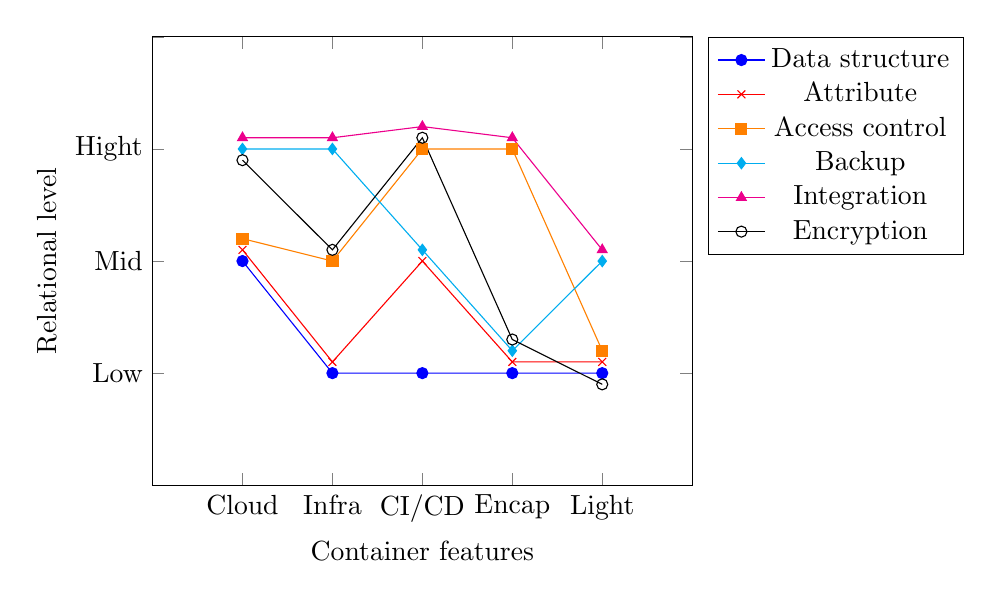
\begin{tikzpicture}
      \begin{axis}[
          xlabel=Container features,
          ylabel=Relational level,
          xmin=0, xmax=60,
          ymin=-1, ymax=3,
          xtick={10,20,30,40,50},
          xticklabels={Cloud, Infra, CI/CD, Encap, Light},
          ytick={0,1,2,3},
          yticklabels={Low, Mid, Hight},
          legend pos=outer north east
        ]
        \addplot[mark=*,blue] plot coordinates {
            (10,1)
            (20,0)
            (30,0)
            (40,0)
            (50,0)
          };
        \addlegendentry{Data structure}

        \addplot[mark=x,red] plot coordinates {
            (10,1.1)
            (20,0.1)
            (30,1)
            (40,0.1)
            (50,0.1)
          };
        \addlegendentry{Attribute}

        \addplot[mark=square*,orange] plot coordinates {
            (10,1.2)
            (20,1)
            (30,2)
            (40,2)
            (50,0.2)
          };
        \addlegendentry{Access control}

        \addplot[mark=diamond*,cyan] plot coordinates {
            (10,2)
            (20,2)
            (30,1.1)
            (40,0.2)
            (50,1)
          };
        \addlegendentry{Backup}

        \addplot[mark=triangle*,magenta] plot coordinates {
            (10,2.1)
            (20,2.1)
            (30,2.2)
            (40,2.1)
            (50,1.1)
          };
        \addlegendentry{Integration}

        \addplot[mark=o,black] plot coordinates {
            (10,1.9)
            (20,1.1)
            (30,2.1)
            (40,0.3)
            (50,-0.1)
          };
        \addlegendentry{Encryption}
      \end{axis}
    \end{tikzpicture}
  \end{frame}

  \begin{frame}{The reason of matrix}
    \begin{itemize}
      \item Data structure: Have some relation in the performance issue.
      \item Attribute (category): Separate into different containers, dynamic CRUD.
      \item Access control: Could be included in infrastructure's routing rule (LSM).
      \item Backup: Reliable (but not saved in long term).
      \item Integration: Separated database needs to integration those caches, rules.
      \item Encryption: Keep your privacy.
    \end{itemize}
  \end{frame}

  \begin{frame}{Why we need the container?}
    The 2FA can solved the traffic of robots.\\
    Back to the key advantage of the container:\\
    \begin{itemize}
      \item Increased portability.
      \item More consistent operation.
      \item CI/CD.
            \begin{itemize}
              \item We can deploy those updates continuously.
            \end{itemize}
      \item Encapsulation.
    \end{itemize}
  \end{frame}

  \begin{frame}{Architecture}
    \centering
    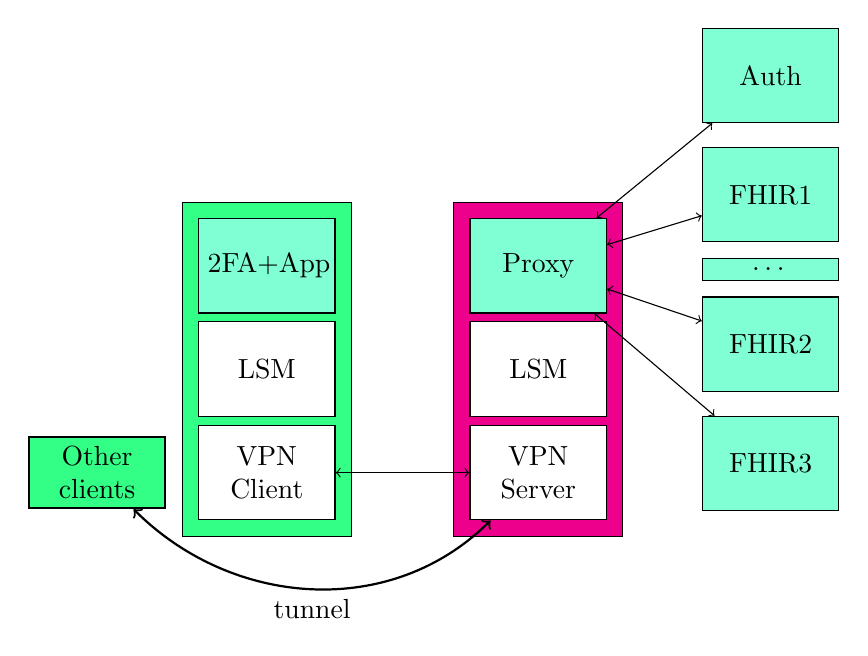
\begin{tikzpicture}
      % Styles
      \tikzstyle{block} = [draw, rectangle, text width=1.5cm, text centered, minimum height=1.2cm, fill=white]
      \tikzstyle{special} = [draw, rectangle, text width=1.5cm, text centered, minimum height=1.2cm, fill=aquamarine]
      \tikzstyle{container} = [draw, rectangle, inner sep=0.2cm, fill=aquamarine2, minimum height=3cm]
      \tikzstyle{ser_container} = [draw, rectangle, inner sep=0.2cm, fill=magenta, minimum height=3cm]
      \tikzstyle{empty} = [draw, rectangle, text width=1.5cm, fill=aquamarine, text centered]
      \tikzstyle{client} = [draw, rectangle, text width=1.5cm, fill=aquamarine2, text centered]
      \def\bottom\#1\#2{\hbox{\vbox to \#1{\vfill\hbox{\#2}}}}
      \tikzset{
        mybackground/.style={execute at end picture={
                \begin{scope}[on background layer]
                  \node[] at (current bounding box.north){\bottom{1cm} \#1};
                \end{scope}
              }},
      }

      \node [special, name=cli_app] {2FA+App};
      \node [block, below=.1cm of cli_app] (cli_lsm) {LSM};
      \node [block, below=.1cm of cli_lsm] (cli_vpn) {VPN Client};
      \node [block, right=1.7cm of cli_vpn] (ser_vpn) {VPN Server};
      \node [block, above=.1cm of ser_vpn] (ser_lsm) {LSM};
      \node [special, above=.1cm of ser_lsm] (ser_proxy) {Proxy};
      \node [special, above right=1.7cm of ser_proxy] (Auth) {Auth};
      \node [special, below=.3cm of Auth] (FHIR1) {FHIR1};
      \node [empty,   below=.2cm of FHIR1] (dots) {\ldots};
      \node [special, below=.2cm of dots] (FHIR2) {FHIR2};
      \node [special, below=.3cm of FHIR2] (FHIR3) {FHIR3};

      \node [client, left=.4cm of cli_vpn, thick] (o_cli) {Other clients};

      \begin{scope}[on background layer, mybackground=Client]
        \node [container,fit=(cli_app) (cli_lsm) (cli_vpn)] (cli) {Client};
      \end{scope}
      \begin{scope}[on background layer]
        \node [ser_container,fit=(ser_proxy) (ser_lsm) (ser_vpn)] (Interface) {Interface};
      \end{scope}
      \draw [<->] (cli_vpn) -- (ser_vpn);
      \path (o_cli) edge [thick, out=-45, in=-135, <->] node[below] {tunnel} (ser_vpn);
      \draw [<->] (ser_proxy) -- (Auth);
      \draw [<->] (ser_proxy) -- (FHIR1);
      \draw [<->] (ser_proxy) -- (FHIR2);
      \draw [<->] (ser_proxy) -- (FHIR3);
    \end{tikzpicture}
  \end{frame}

  \begin{frame}{Pros and crons}
    \begin{itemize}
      \item Pros:
            \begin{itemize}
              \item Solved the malicious flow.
              \item Truly people authorization.
              \item Coupled with Taiwan healthcare system.
            \end{itemize}
      \item Crons:
            \begin{itemize}
              \item Modified kernel.
              \item Slower.
              \item Coupled with OS.
            \end{itemize}
    \end{itemize}
  \end{frame}

  \begin{frame}{With the container security issue}
    \begin{itemize}
      \item The trend of micro-service on cloud computing.
      \item CI/CD.
      \item Encapsulation.
    \end{itemize}
    Still not solved:
    \begin{itemize}
      \item Hooked glibc.
      \item Composed system calls (LSM).
    \end{itemize}
  \end{frame}

  \begin{frame}{Reference}
    \href{https://wiki.gentoo.org/wiki/Wireguard}{Wireguard kernel module}
  \end{frame}

\end{CJK*}
\end{document}